\documentclass[9pt,twocolumn,twoside]{styles/osajnl}
\usepackage{fancyvrb}
\journal{i524} 

\title{RabbitMQ}

\author[1,*]{Abhishek Gupta}

\affil[1]{School of Informatics and Computing, Bloomington, IN 47408, U.S.A.}

\affil[*]{Corresponding authors: abhigupt@iu.edu}

\dates{project-001, \today}

\ociscodes{Cloud, I524}

% replace this with your url in github/gitlab
\doi{\url{https://github.com/cloudmesh/sp17-i524/blob/master/paper1/S17-IO-3005/report.pdf}}

\begin{abstract}
RabbitMQ provides simple yet powerful messaging platform which allows applications pass messages in a reliable and fault tolerant way. RabbitMQ implements Advanced Message Queuing Protocol (AMQP) and is written in Erlang programming language. It runs on all major operating systems and supports SDK in all major programming languages\cite{www-rabbitmq-develop} including objective-C, swift and node.js. When we look for messaging, we look for certain features: asynchronous messaging, large scale, reliability, clustering, multi-protocol, highly available, fault tolerant. RabbitMQ\cite{www-rabbitmq-pivotal} fulfills these requirements and provides a distributed, persistent, highly available, fault tolerant messaging system which can scale as data grows.
\newline
\end{abstract}

\setboolean{displaycopyright}{true}

\begin{document}

\maketitle

\section{Introduction}

RabbitMQ based\cite{www-rabbitmq-pivotal} off AMQP (Advanced Message Queuing Protocol\cite{vinoski2006advanced}) Which defines how client applications connect to message brokers. Message brokers receive messages from producers and make it available to consumers. The producer  posts messages to exchanges and broker agent reads these messages from exchange and writes to queues. Consumers can further read messages from the queue. It also supports a notion of acknowledgements where consumers can post an acknowledgement back to broker and which in turn can post messages back to the producer. 

Looking back at the history\cite{videla2012rabbitmq} of development of rabbitMQ, it started with IBM MQseries in 1993, 1997 Microsoft MQ, 2001 java messaging service. It was in 2003 where JPMorgan created the first version AMQP which became the base for RabbitMQ technologies formed in 2006.

\begin{figure}[htbp]
\centering
\fbox{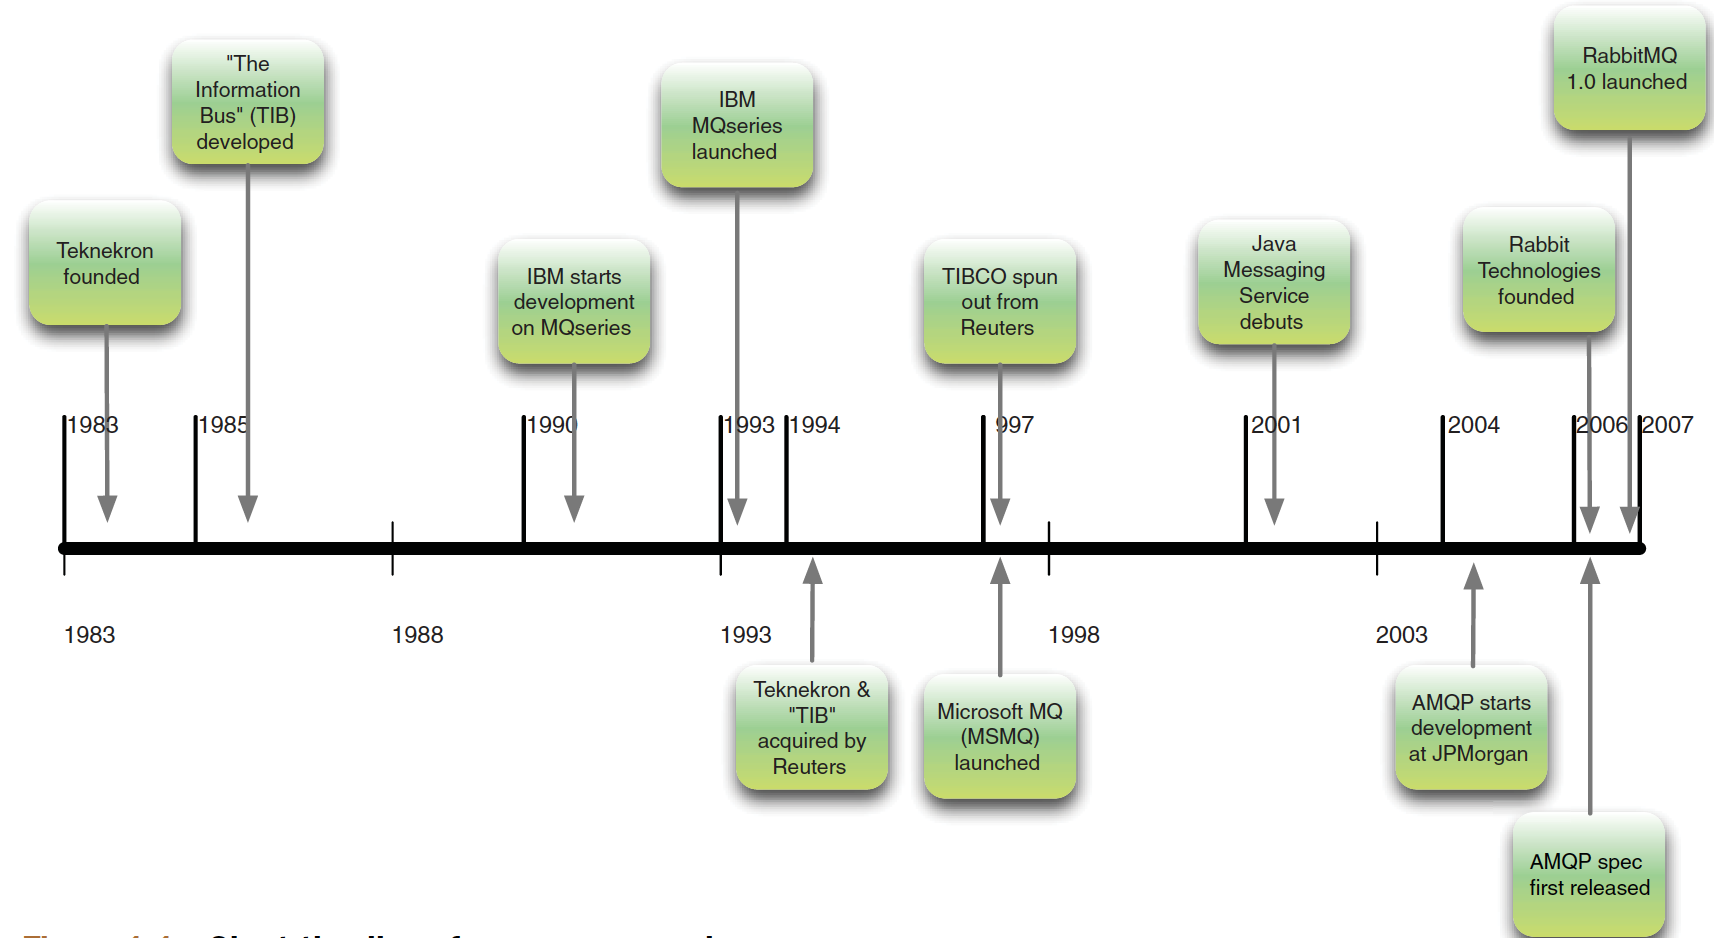
\includegraphics[scale=0.2]{images/mq_timeline}}
\caption{Timeline for evolution of RabbitMQ}\cite{videla2012rabbitmq}
\label{fig:false-color}
\end{figure}


\section{Architecture}

\cite{videla2012rabbitmq}At high level, producer publishes the message to the broker. Consumer consumes or subscribes the messages from the broker. Broker is the middle man who has the knowledge of exchanges and queues. It maintains the bindings between exchanges and queues. The consumers read the messages from the queue. Following table shows different exchanges supported by RabbitMQ and corresponding default exchanges\cite{www-rabbitmq-pivotal} .

\begin{center}
 \begin{tabular}{||c c||} 
 \hline
 Name & Default pre-declared names \\ [0.5ex] 
 \hline\hline
 Direct exchange & (Empty string) and amq.direct  \\ 
 \hline
 Fanout exchange & amq.fanout  \\
 \hline
 Topic exchange & amq.topic  \\
 \hline
 Headers exchange & amq.match (and amq.headers in RabbitMQ) \\
 \hline
\end{tabular}
\end{center}

\section{Type of exchanges}
\label{sec:examples}

The sections below explains various types of exchanges supported by RabbitMQ.

\subsection{Default Exchange}

It is created by the broker and all queues are bound to default exchange unless specified separately. For example we have a queue called demoqueue, all messages assigned to demoqueue will be routed by default exchange.

\subsection{Direct exchange}

It is used to route messages to queue with a given routing key. For example a message queue has routing key K. A message with same routing key K will be delivered to same message queue.

\subsection{Fanout exchange}

Delivers messages to all queues that are bound to a given exchange ignoring the routing key. For example if there are 5 queues bound to a exchange E. Messages to exchange E are delivered to all 5 queues.

\subsection{Topic exchange}

It delivers the messages to a given queue, not just based on the routing key but a pattern specified in the message called topic. It can be useful in scenario when consumer/application decides to which topic(s) it is interested in. Further, it can subscribe to those topics(or messages).

\subsection{Header exchange}

This exchange ignores the routing key but uses the header parameter to decide which messages goes to which queue. A message is matched when a value in header matches with the one specified in the queue binding.
Exchanges have other important attributes apart from routing key and exchange type for example name, durability, auto-delete, arguments etc. Durability allow messages to persist on disk in case of broker restarts. Auto-delete deletes the exchange, once all queue have finished using the exchange.

\begin{figure}[htbp]
\centering
\fbox{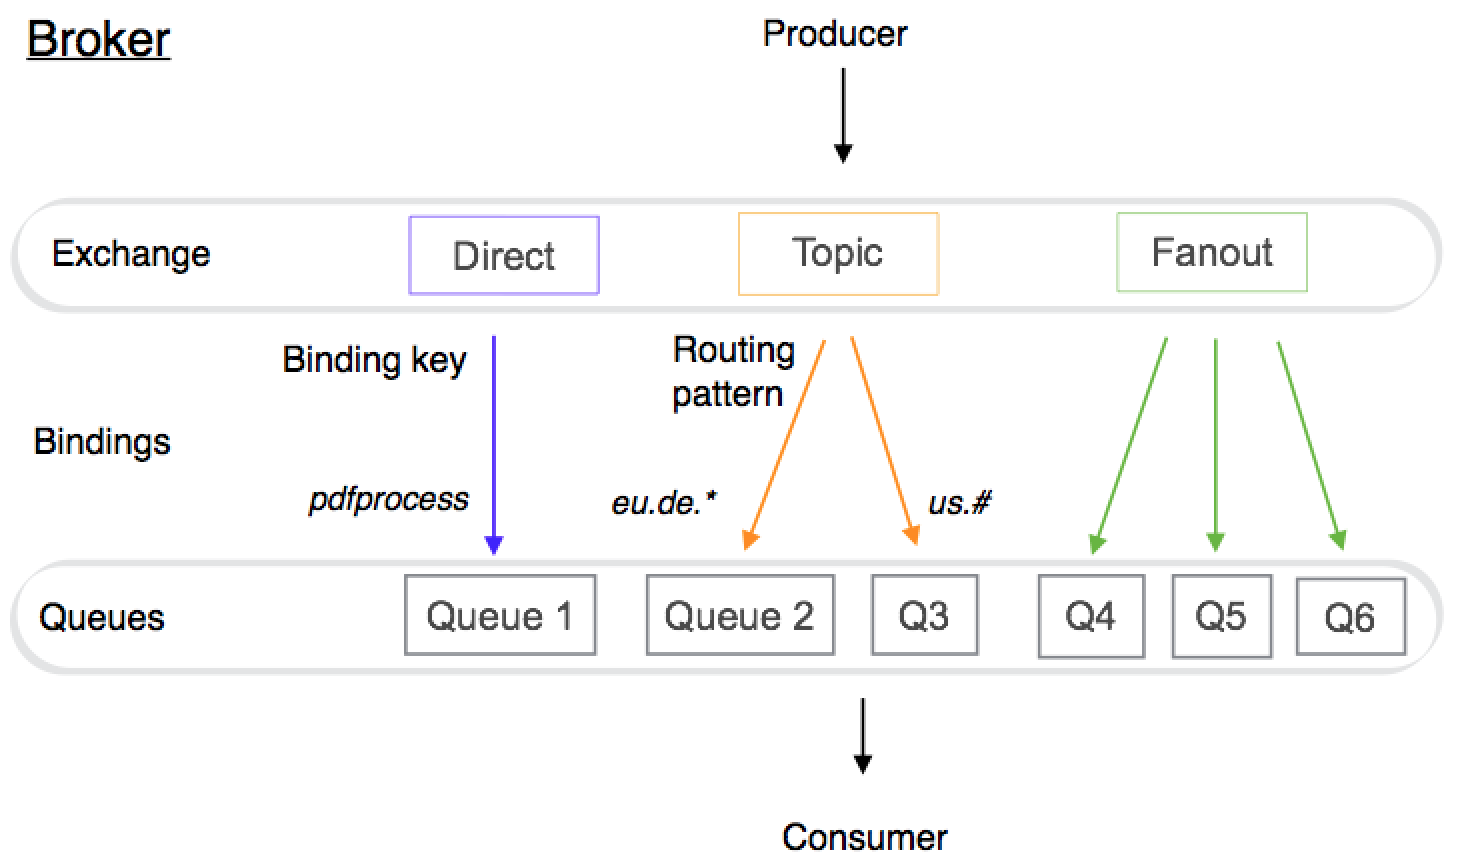
\includegraphics[scale=0.3]{images/exchanges-topic-fanout-direct}}
\caption{Different type of exchanges supported by RabbitMQ}\cite{www-rabbitmq-Johan}
\label{fig:false-color}
\end{figure}

\section{Bindings}

Bindings are the rules that define how exchanges will route messages to the queue. To route all messages from exchange E to queue Q, Q has to be bound to Exchange E. Bindings use routing key as one of the criteria to route messages to a queue. However, routing key is optional and not always applicable.

\section{Consumers}

Messages from message queue are eventually used or consumed by consumers. Consumers can use push or pull mechanism to consume these messages. Push API have messages delivered to the consumer whereas a Pull API is used to fetch messages from the queue. 

\section{Message Acknowledgement}

It has a built-in mechanism to send and receive acknowledgements. Producer can send messages and wait to acknowledgement in the response queue from consumer. Consumer can receive messages and post acknowledgement to response queue. Here request queue and request exchange can be used to send and receive messages. Whereas response queue and response exchange can be used to send and receive acknowledgements. This mechanism makes RabbitMQ robust in case of failures.

\section{Clustering}

\cite{videla2012rabbitmq}To achieve high availability and making sure producers and consumers send and receive data without knowing about node failures, clustering was introduced. RabbitMQ follows OTP(open telecom platform) framework provided by erlang to achieve high availability. RabbitMQ by default doesn't replicate the content of queues i.e. all queues are stored on one node in the cluster. To achieve clustering rabbitmq keeps track of metadata for queue, exchange, binding and vhost. In case of cluster, it only stores all information about the queue like metadata, state and contents on one node rather than all nodes in the cluster. However, it stores metadata and pointer to actual data on each node in the cluster. This is to optimize storage space and performance. 

\begin{figure}[htbp]
\centering
\fbox{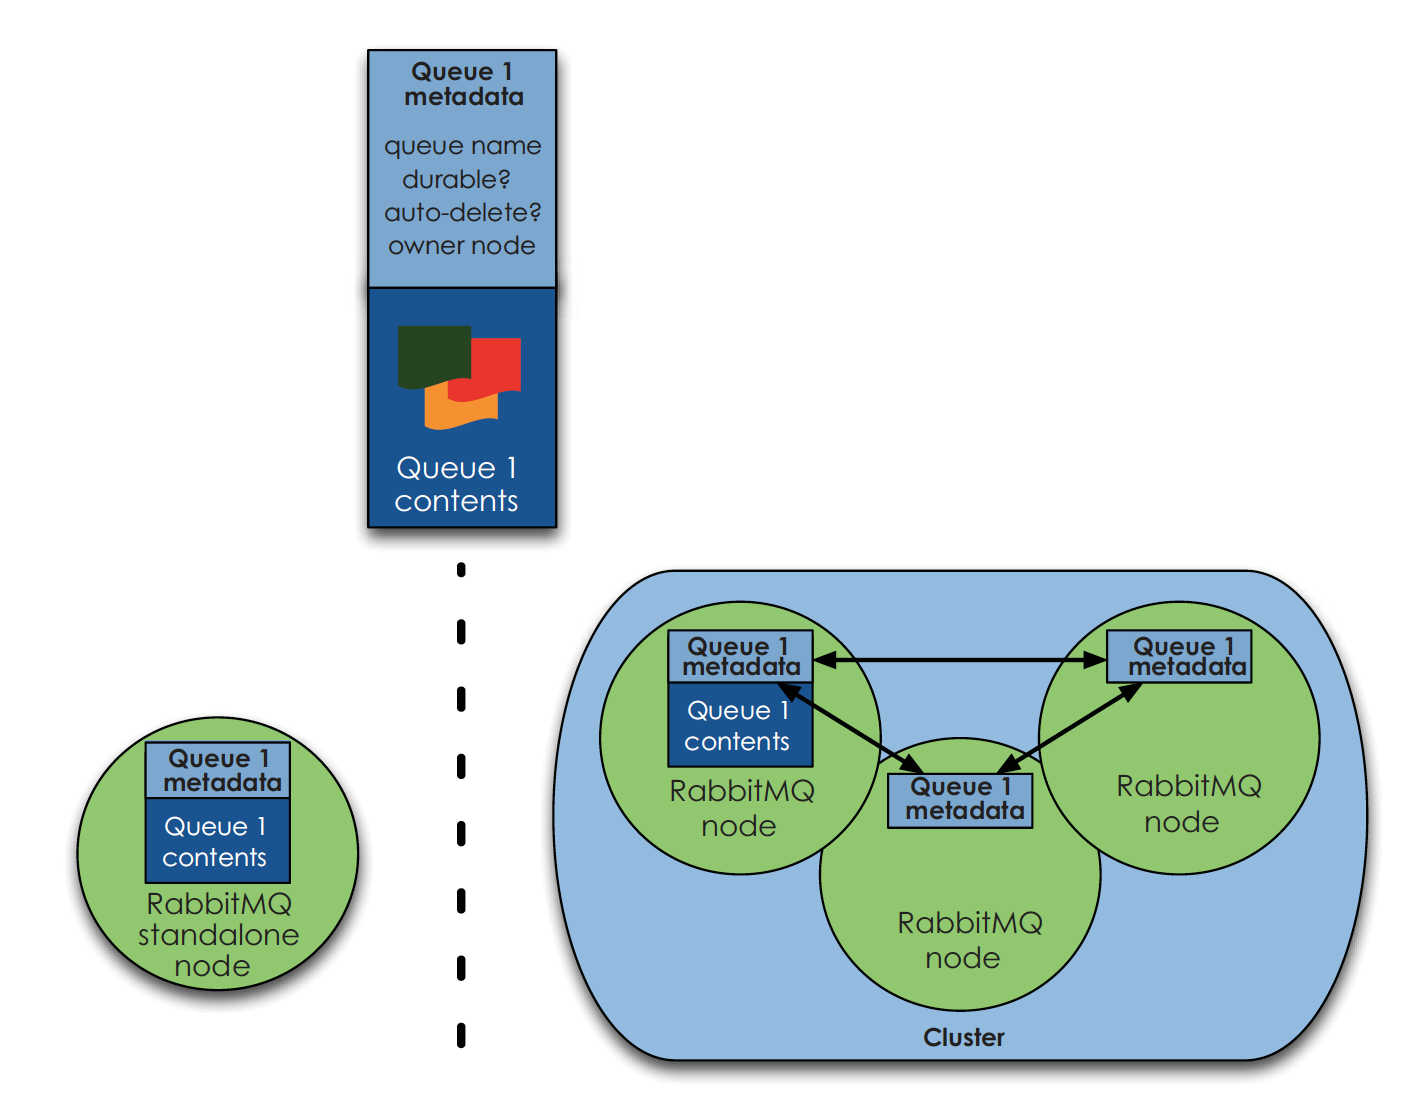
\includegraphics[width=\linewidth]{images/clustering-queue-metadata}}
\caption{Shows queue metadata for a cluster vs single node}\cite{videla2012rabbitmq}
\label{fig:false-color}
\end{figure}

On the other hand exchanges are just bindings to the queues. So when you send a message to rabbitmq exchange, the channel checks the routing key of the message and compares it against the queue bindings. Further it sends the message to appropriate queue. Since, exchanges are just lookup tables for queue bindings, they are replicated across all nodes on the cluster. 

\section{Management}
RebbitMQ provides all management using:
\begin{itemize}
	\item  web ui 
	\item REST interface
	\item Rabbitmqctl command line utility
\end{itemize}

Web UI can be used by administrators to create user, monitor queues and exchanges, view statistics, add configurations etc. Similar functionality can be achieved by cli utility rabbitmqctl and REST API. Rabbitmqctl can be used to automate rabbitmq deployments and management. IT can also be used to write automated tests. REST Api can used for integrating with 3rd part UI and plugins. Using REST api you can monitor the number of connections, download or upload a configuration, list the nodes in the cluster, create or delete rabbitmq users, view or create virtual host, set permission for a user etc. You can also list all current APIs using following url: http://localhost:55672/api with some api documentation and explanations.

\begin{figure}[htbp]
\centering
\fbox{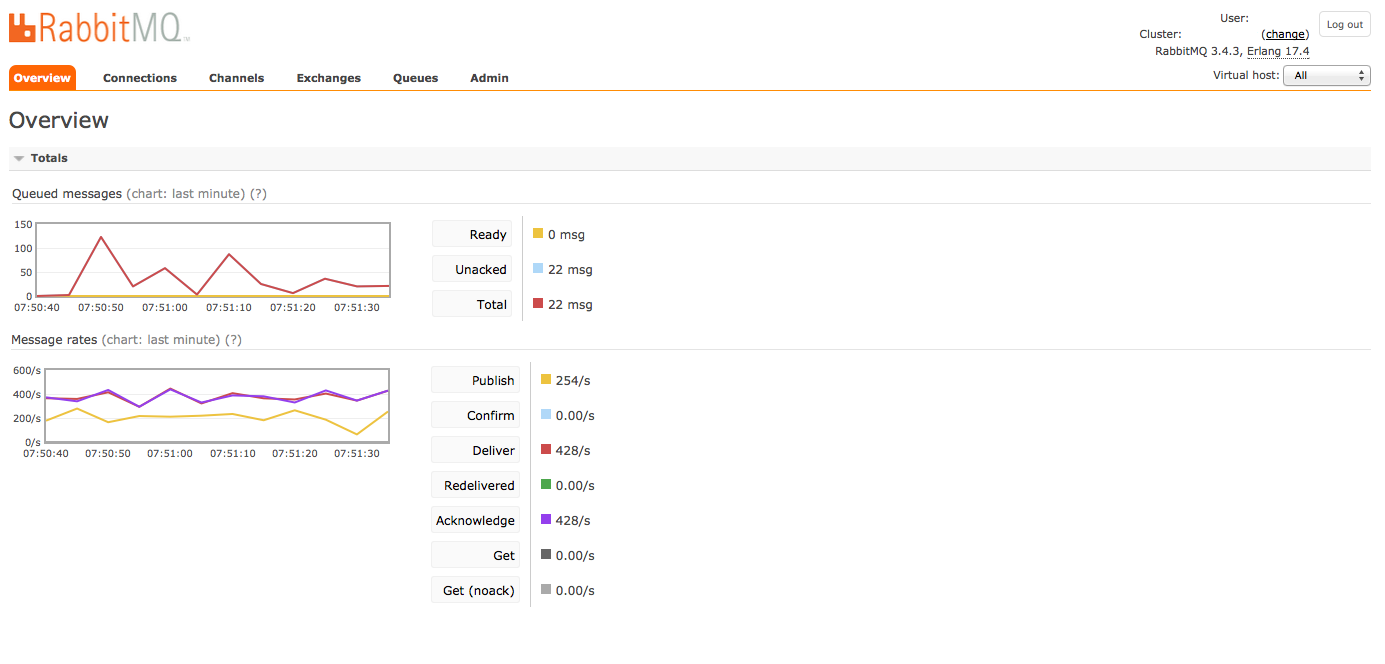
\includegraphics[width=\linewidth]{images/rabbitmq-monitoring.png}}
\caption{RabbitMQ management UI showing messages queued and message data rates}\cite{www-rabbitmq-Johan}
\label{fig:false-color}
\end{figure}

\section{Licensing}
RabbitMQ is licensed under \href{https://www.rabbitmq.com/mpl.html} {Mozilla Public License(MPL) and GPL v2}. \cite{www-rabbitmq-pivotal}

\section{Use Cases}

RabbitMQ messaging can be useful in applications which require asynchronous messaging for example an application initiates a task by posting a message to RabbitMQ, it doesn't have to wait for the task to get completed. Rather it can periodically check the status of task. It can be useful to scale up as the data volume grows by adding additional nodes to RabbitMQ cluster. With distributed applications where applications run as micro-services in a container or virtual machine, RabbitMQ is useful to communicate and share data between different services. RabbitMQ can be managed separately with its management UI, CLI tool and REST api interface. This decouples the messaging layer from application and makes the overall design very robust. 

\section{Conclusion}
RabbitMQ is an open source platform and provides a robust messaging platform for applications. It provides simple manageability decoupling with the application. RabbitMQ can scale well when application demand increases and can handle more data by adding more nodes to the cluster. Based on test \cite{jones2011rabbitmq}conducted on RabbitMQ with set of 4K(4096) and 16K(16384) messages, the performance of RabbitMQ on multi node cluster decreases in comparison with single node cluster to reach a threshold and then becomes stable. This decrease in performance can be primarily accounted due to replication between nodes in the cluster.These tests were conducted on combination of single publisher and single subscriber, multiple publishers and single subscriber, multiple publishers and multiple subscribers but there is no concrete conclusion to these test and numbers.

\section*{Acknowledgements}
Special thanks to Professor Gregor von Laszewski, Dimitar Nikolov and all associate instructors for all help and guidance related to latex and bibtex, scripts for building the project, quick and timely resolution to any technical issues faced. The paper is written during the course  {I524: Big Data and Open Source Software Projects, Spring 2017} at Indiana University Bloomington.

 
\medskip

% Bibliography
% \bibliographystyle{unsrt}
\bibliography{references}

\end{document}
